\chapter{Kata Containers}
\label{chapter:katacontainers}

Securing container runtime is a crucial task in MEC in order to run multiple instances in the same edge securely. Container escapes are exposing other instances in the platform. Therefore, multiple solutions to provide stronger workload isolation using hardware virtualization technology as a second layer of defense have been developed. One of the most prominent approach includes wrapping the container inside a micro VM, which is a lightweight version of traditional VM with minimal overhead. The dedicated kernel of micro VM, provides isolation of network, I/O and memory and can utilize hardware-enforced isolation with virtualization extensions. In this Thesis, we will focus on Kata Containers as a secure container runtime. Kata Containers perform like containers, but provide the workload isolation and security advantages of VMs. It combines the benefits of containers and VMs. \cite{KataContainers}

Kata Containers has originated from Intel's Clear Containers \cite{ClearContainers} and Hyper runV \cite{runV} in December 2017. KC is open source and licensed under the Apache 2.0 license. The development is driven by an Architecture Committee. This committees members are elected by contributors, oversees architectural decisions, including standardization, and resolves technical disagreements between project maintainers. Currently this committee is comprised of five members from Apple, Intel, Ant Financial, and Red Hat. \cite{KataContainersGovernance} \cite{KataContainers}

\section{Architecture}

In this Thesis environment, Kata Containers is deployed within Kubernetes. Figure \ref{fig:KataContainersArchitecture} demonstrates the latest architecture defined version 2.0.0. The architecture is comprised of six elements: Kubernetes, CRI-O, Kata Shim V2, Hypervisor, Agent, and Virtual Machine.

\subsection{Kubernetes}

Kubernetes acts as an container-orchestration system for automating deployment, scaling, and management of containerized applications \cite{Kubernetes}. Kubernetes offers flexible configuration and it can installed inside a VM or on bare-metal. Like most distributed computing platforms, a Kubernetes cluster consists of at least one master node and multiple compute nodes. Each node runs a container runtime, such as Docker or Kata Containers, along with an agent that communicates with the master.

Each container is launched as a pod. Pods are the atomic unit on the Kubernetes platform. A single node can include multiple pods inside it, and each pod is tied to the node it is created within. Runtime can be selected on a pod level, thus a single node can consists of workloads with various runtimes. This comes handy, whenever non-confidential, but highly performance centric application needs to be within more security oriented applications.

\subsection{CRI-O}


\subsection{Kata Shim V2}

\subsection{Agent}

Agent, also known as Kata-Agent, run inside the Kubernetes pod and

\subsection{Hypervisor}

Kata Containers currently supports two/three different hypervisors: KVM, QEMU, and Firecracker.




  



\begin{figure}[ht]
  \begin{center}
    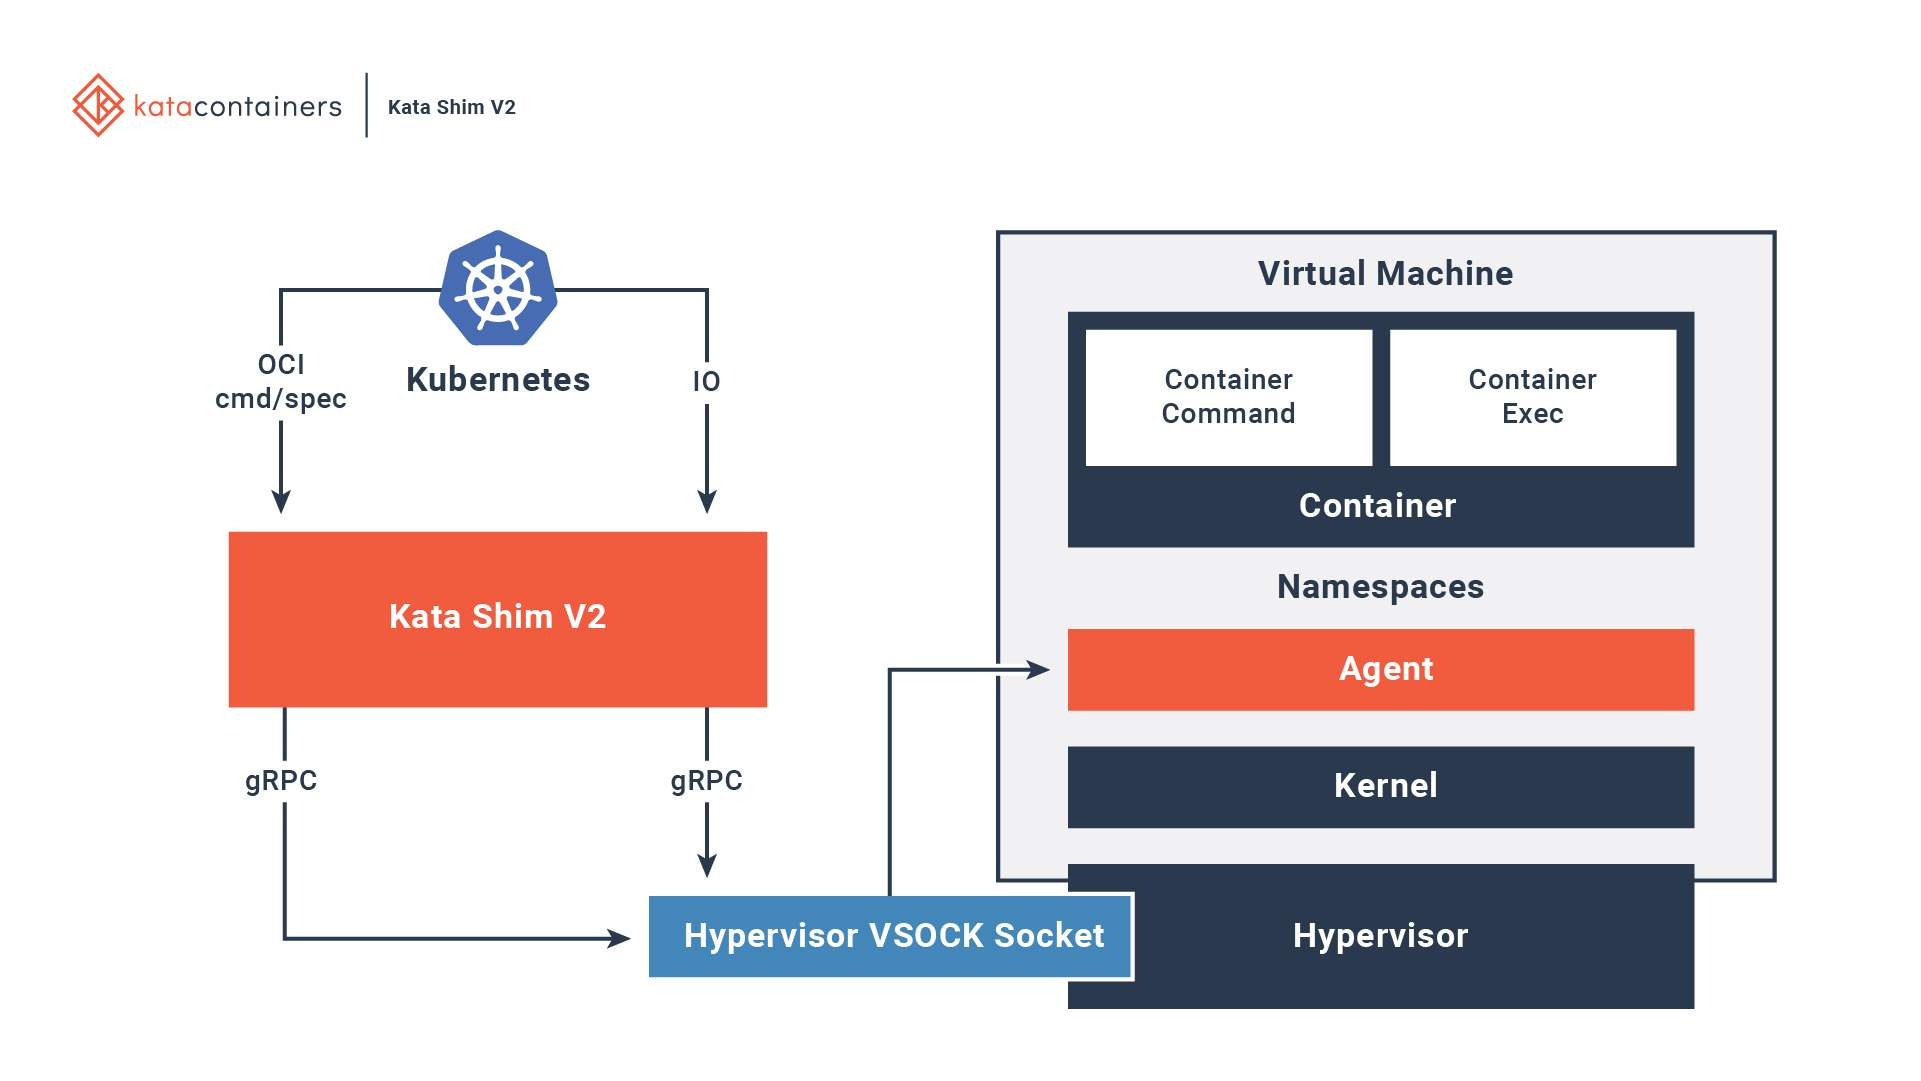
\includegraphics[width=15cm]{LaTeX/images/KataContainersArchitecture.jpg}
    \caption{Kata Containers 2.0 architecture \cite{KataContainers}}
    \label{fig:KataContainersArchitecture}
  \end{center}
\end{figure}


\begin{figure}[ht]
  \begin{center}
    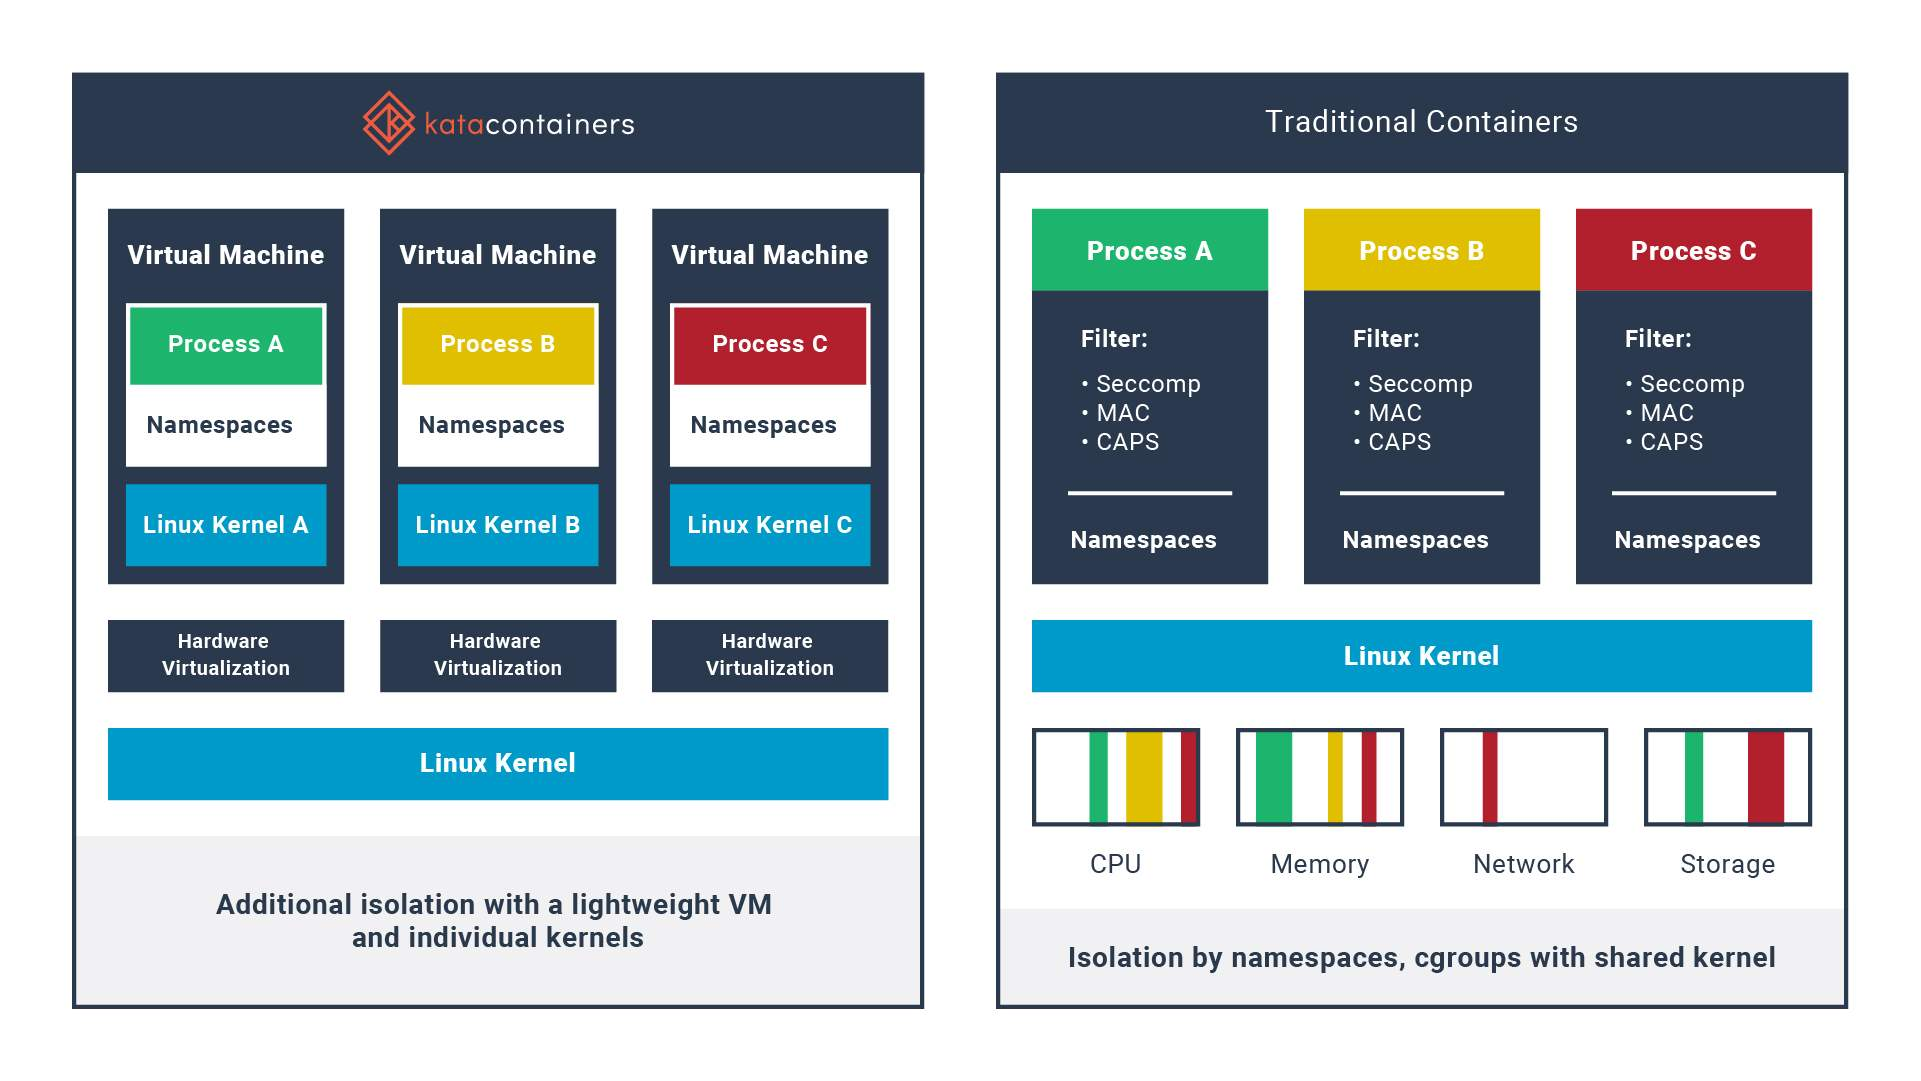
\includegraphics[width=14cm]{LaTeX/images/KataContainersStack.jpg}
    \caption{Kata Containers stack vs traditional container stack\cite{KataContainers}}
    \label{fig:KataContainersStack}
  \end{center}
\end{figure} 

Each Kubernetes pod is wrapped inside its own lightweight VM, thus isolating workloads even from the same host or container maintainer.




Kata Containers is Open Container Initiative (OCI) compliant runtime, thus it obeys OCI runtime specification and supports all the OCI runtime operations. As any OCI compliant runtime, the KC works seamlessly with the Kubernetes Container Runtime Interface (CRI) through the CRI-O and Containerd implementation. The isolation is achieved with QEMU \cite{QEMU} or Kernel-based Virtual Machine (KVM) \cite{KVM} for pod that \texttt{kubelet} in Kubernetes creates respectively.

\section{Networking}

\section{Related work}

Kata Containers is not the sole option providing secure container runtime nor isolation in the container kernel layer. Amazon Web Services (AWS) uses their in-house built Firecracker runtime, which uses KVM to launch workload in lightweight micro-virtual machines. Of Amazon's cloud products, Firecracker is deployed at least in AWS Lambda and Fargate. Firecracker currently supports Intel CPUs, with AMD and Arm support in developer preview. Firecracker microVM's are also integrated with other runtimes such as containerd and Kata Containers. \cite{AWS}\cite{Debab2021}\cite{FirecrackerDesign}

Microsoft offers a container instance isolation option inside Azure with Hyper-V. The hardware isolation is based on VMs, likewise in KC and Firecracker, thus leveraging the additional kernel layer. \cite{Hyper-V}

gVisor provides a second isolation method, differing from Kata Containers and Firecracker. gVisor intercepts application system calls and acts as the guest kernel without translating through virtualized hardware. The architecture can be thought of as a merged kernel and Virtual Machine Manager (VMM). gVisor includes OCI runtime runsc, which provides the isolation boundary between the application and host kernel. Google develops gVisor, and it is harnessed in various Google's cloud products such as Kubernetes Engine \cite{GKE} and Cloud Run \cite{CloudRun}. \cite{Debab2021}\cite{gVisor}

A third approach for container isolation is IBM Nabla\cite{Nabla}. Nabla containers use library OS, also known as unikernel, to avoid system calls and reduce the attack surface. Nabla is based on a custom VMM named Nabla Tender to manage lightweight VMs executing unikernels. Nabla containers only use seven system calls, blocking all others via a Linux \texttt{seccomp} policy. The Nabla Tender intercepts hypercalls related to storage and network from unikernel VMs and translates them into syscalls to the host. \cite{Debab2021}

All the before-mentioned projects are open source and actively maintained. However, Nabla seems to be slightly less active in comparison to the other projects. Commercial and enterprise cloud platforms, such as AWS, uses Firecracker, and GKE uses gVisor. However, it is unknown for security reasons which approaches are used in the other platforms to isolate containers.


% that it fits to the same space as the text (total width = \textwidth).
% If you do need more space, you can either
% 1) ignore the LaTeX warnings 
% 2) use the textpos-package to manually position the table (read the package
%    documentation)
% 3) if you have the table as a PDF document (of correct size, A4), you can use
%    the pdfpages package to include the page. This overrides the margin
%    settings for this page and LaTeX will not complain.
% ------------------------------------------------------------------
% Another note:
% ------------------------------------------------------------------
% If your table fits to \textwidth, but the cells are so narrow that the text
% in p{..}-formatted cells does not flow nicely (you get underfull warnings 
% because LaTeX tries to justify the text in the cells) you can manually set
% the text to unjustified by using the \raggedright command for each cell 
% that you do not want to be justified (see the example below). \raggedleft 
% is also possible, of course...